% -*- root: main.tex -*-
%-------------------------------------------------------------------------------
\chapterimage{chapter_head_2.pdf} 

%-------------------------------------------------------------------------------
\chapter{ROS 설치 (일반PC)}

%-------------------------------------------------------------------------------
\section{ROS Indigo 설치}\index{ROS Indigo 설치}

%-------------------------------------------------------------------------------
\subsection{개발 환경}\index{개발 환경}

본 강좌는 아래와 같은 개발 환경에서 ROS 설치를 설명한 글이다. ROS는 Ubuntu, OS X, Windows, Fedora, Gentoo, OpenSUSE, Debian, Arch Linux 등을 지원하고 있지만 Ubuntu 를 제외하고는 공식적으로 지원하는 것이 아닌 설치 방법만 언급하고 있다. 하지만, 우분투이외의 주요 운영체제인 OS X, Windows 는 유저들이 많은 편이라 어느정도 만족스럽게 쓸 수 있을 것이다. 우분투 버전이 다른 경우에는 공식 페이지\footnote{http://wiki.ros.org/indigo/Installation/Ubuntu}를 보기를 권하며, OS X\footnote{http://wiki.ros.org/indigo/Installation/OSX/Homebrew/Source}, Windows\footnote{http://wiki.ros.org/hydro/Installation/Windows}의 경우에는 각각의 설치 방법을 관련 위키\footnote{ROS 위키, "환경설정", http://wiki.ros.org/ROS/Tutorials/InstallingandConfiguringROSEnvironment}\footnote{ROS 위키, "catkin 빌드 시스템", http://wiki.ros.org/catkin}에서 확인하기 바란다. 여기서는 우분투에 대해서만 언급하겠다.

\begin{itemize}
\item 하드웨어: INTEL 및 AMD 칩을 사용하는 데스크톱 및 노트북 
\item 운영체제: Ubuntu 14.04 LTS (Trusty Tahr)
\item ROS: Indigo Igloo
\end{itemize}

\begin{figure}[h]
\centering
\includegraphics[height=30mm]{pictures/chapter2/ubuntu_14_04.jpg}
\centering
\includegraphics[height=30mm]{pictures/chapter2/indigo_igloo.png}
\caption{우분투 Trusty 버전과 ROS Indigo 버전의 로고}
\end{figure}


%-------------------------------------------------------------------------------
\subsection{ROS Indigo 설치 방법}\index{ROS Indigo 설치 방법}
\label{sec:ROSInstallation}

\begin{exercise}[간단 설치]
아래의 강좌보다 간단히 설치 할 수 있는 스크립트를 이용한 설치 방법은 \ref{sec:SimpleInstallation}[ROS Indigo 간단 설치]을 참조하기 바란다.
\end{exercise}

%-------------------------------------------------------------------------------
\subsubsection{NTP (Network Time Protocol) 설정}
ROS 공식 설치항목에는 포함되어 있지는 않지만 NTP 설정을 해주므로써 서로 다른 PC간의 통신에서 ROS Time 의 오차를 줄이기 위하여 NTP 설정을 해주도록 하자. 설정법은 매우 간단한데, 아래의 명령어처럼 우선 chrony 를 설치한 후, ntpdate 라는 명렁어로 ntp 서버를 지정하면 된다. 결과, 서버측과의 현재 컴퓨터 시간 오차를 표시해주며, 서버 시간에 맞추게 될것이다. 이는 서로 다른 PC 간에 같은 NTP 서버를 지정함으로써 시간오차를 최소한으로 줄이는 방법이라 할 수 있다.

\begin{lstlisting}[language=bash]
sudo apt-get install chrony
sudo ntpdate ntp.ubuntu.com
\end{lstlisting}

%-------------------------------------------------------------------------------
\subsubsection{소스 리스트 추가}
"sources.list"에 ROS 저장소 주소를 추가하자. 새로운 커맨드 창을 열고 아래와 같이 입력한다. 

\begin{lstlisting}[language=bash]
sudo sh -c 'echo "deb http://packages.ros.org/ros/ubuntu trusty main" > /etc/apt/sources.list.d/ros-latest.list'
\end{lstlisting}

%-------------------------------------------------------------------------------
\subsubsection{키 설정}
ROS 저장소로부터 패키지를 다운로드 받기위해 공개키를 추가하자. 아래와 같이 입력한다.

\begin{lstlisting}[language=bash]
wget https://raw.githubusercontent.com/ros/rosdistro/master/ros.key -O - | sudo apt-key add -
\end{lstlisting}

%-------------------------------------------------------------------------------
\subsubsection{패키지 인덱스 업데이트}
소스 리스트에 ROS 저장소 주소를 넣었으니 패키지 리스트를 다시 재인덱싱을 하고, 설치상에 필수 사항은 아니지만 ROS설치전에 현재 설치된 우분투 관련 모든 패키지를 판올림 하기를 추천한다.

\begin{lstlisting}[language=bash]
sudo apt-get update && sudo apt-get upgrade
\end{lstlisting}

%-------------------------------------------------------------------------------
\subsubsection{ROS Indigo Igloo 설치}
이 명령어로 데스크톱용 기본적인 ROS 패키지들을 설치하게 된다. 여기에는 ROS, rqt, rviz, 로봇 관련 라이브러리, 시뮬레이션, 네이게이션 등이 포함되어 있다.

\begin{lstlisting}[language=bash]
sudo apt-get install ros-indigo-desktop-full
\end{lstlisting}

필자의 경우에는 추가로 rqt 관련 패키지를 설치하고 있다. 위의 설치만으로도 기본적인 rqt는 포함되지만 아래의 설치로 rqt관련 모든 패키지를 설치하는것이 여러모로 편하고, 다양한 rqt 플러그인을 사용가능해진다.

\begin{lstlisting}[language=bash]
sudo apt-get install ros-indigo-rqt-*
\end{lstlisting}

만약, 그 이외에 패키지를 설치하고 싶은 경우에는 아래와 같이  "apt-cache" 의 명령어를 이용하여 "ros-indigo" 로 시작되는 패키지들을 검색할 수 있다. 현재 아래의 명령어를 실행해보면 대략 800여개의 패키지를 확인할 수 있다. 패키지 개별 설치를 원하는 경우에는 "sudo apt-get install ros-indigo-[패키지이름]" 과 같은 명령어로 개별 패키지를 설치 가능하다. 그 이외에 GUI 툴인 sysnaptic package manager 를 이용해도 된다.

\begin{exercise}[APT (Advanced Packaging Tool)]
apt-get, apt-key, apt-cache 등의 나오는 apt는 Advanced Packaging Tool 이라고 하여서 우분투(Ubuntu)를 포함안 데비안(Debian)계열의 리눅스에서 사용하는 패키지 관리 명령어이다\footnote{http://en.wikipedia.org/wiki/Advanced\_Packaging\_Tool}.
\end{exercise}

\begin{exercise}[패키지 검색 방법]
apt-cache search ros-indigo
\end{exercise}

\begin{exercise}[패키지 개별 설치 방법]
sudo apt-get install ros-indigo-패키지이름
\end{exercise}

\begin{exercise}[이전 버전의 ROS 삭제 및 번갈아 가며 사용하기]
아래의 명령어로 설정과 파일을 같이 삭제 가능하다. 만약, 기존 버전과 함께 사용하고자하는 경우에는 설정파일을 불러오는 명령어중 source /opt/ros/indigo/setup.bash 의 부분을 indigo 또는 hydro 로 바꾸면 된다. sudo apt-get purge ros-hydro-*
\end{exercise}

%-------------------------------------------------------------------------------
\subsubsection{rosdep 초기화}
ros를 사용하기전에 rosdep 를 초기화 해주어야만 한다. rosdep 는 ros의 핵심 컴포넌트 들을 사용하거나 컴파일 할때 의존성 패키지를 쉽게 설치하여 사용자 편의성을 높인 기능이다.

\begin{lstlisting}[language=bash]
sudo rosdep init
rosdep update
\end{lstlisting}

%-------------------------------------------------------------------------------
\subsubsection{rosinstall 설치}
ros의 다양한 패키지를 인스톨하는 프로그램이다. 빈번하게 사용할 정도로 유용한 툴인만큼 꼭 설치하도록 하자. 

\begin{lstlisting}[language=bash]
sudo apt-get install python-rosinstall
\end{lstlisting}

%-------------------------------------------------------------------------------
\subsubsection{환경설정 파일 불러오기}
환경설정이 설정되어 있는 파일을 불러온다. ROS\_ROOT, ROS\_PACKAGE\_PATH 등의 환경 변수들이 정의되어 있다.

\begin{lstlisting}[language=bash]
source /opt/ros/indigo/setup.bash
\end{lstlisting}

%-------------------------------------------------------------------------------
\subsubsection{작업폴더 생성 및 초기화}
ROS에서는 catkin 이라는 ROS 전용 빌드 시스템을 사용하고 있다. 이를 사용하기위해서는 아래와 같이 catkin 작업 폴더 및 작업 폴더 초기화 설정을 해주어야 한다. (아래의 설정은 ROS를 사용함에 있어서 한 번만 해주면 된다.)

\begin{lstlisting}[language=bash]
mkdir -p ~/catkin_ws/src
cd ~/catkin_ws/src
catkin_init_workspace
\end{lstlisting}

catkin 작업 폴더를 생성하였으면 컴파일을 하자. 현재의 catkin 작업 폴더에는 src폴더 및 그 안의 CMakeLists.txt 이외에 아무런 파일이 없지만 테스트삼아 아래와 같이 "catking\_make"명령어를 이용하여 빌드하여 보자. 

\begin{lstlisting}[language=bash]
cd ~/catkin_ws/
catkin_make
\end{lstlisting}

문제없이 빌드를 마치게 되면 아래와 같이 "ls" 명령어를 실행해보자. 유저가 직접 생성하였던 "src" 폴더 이외의 없었던 "build" 및 "devel"폴더가 새로 생성되었다. catkin 빌드 시스템의 빌드 관련 파일은 "build" 폴더에, 빌드 후 실행관련 파일은 "devel" 에 저장되게 된다.

\begin{lstlisting}[language=bash]
ls
build  devel  src
\end{lstlisting}

마지막으로, catkin 빌드 시스템과 관련된 환경 파일을 불러오자. 

\begin{lstlisting}[language=bash]
source ~/catkin_ws/devel/setup.bash
\end{lstlisting}

%-------------------------------------------------------------------------------
\subsection{환경 설정}\index{환경 설정}

위 설치과정에서 사용된 아래 명렁어처럼 환경 설정 파일을 불러오는 것은 새로운 터미널 창을 열때마다 매번 실행해줘야 한다. 이러한 번거로운 작업을 없애기 위하여 새로운 터미널 창을 열때마다 정해진 환경 설정 파일을 읽어오도록 설정해주도록 하자. 또한, ROS 네트워크 설정 및 자주 사용하는 명령어를 단축 명령어로 설정하도록 하자.

\begin{lstlisting}[language=bash]
source /opt/ros/indigo/setup.bash
source ~/catkin_ws/devel/setup.bash
\end{lstlisting}

우선, gedit 프로그램과 같은 문서편집 프로그램을 사용하여 bashrc 파일을 수정하도록 하자. 아래의 명령어로 bashrc 파일을 불러오자.

\begin{lstlisting}[language=bash]
gedit ~/.bashrc
\end{lstlisting}

bashrc 파일을 불러오면 이미 매우 많은 설정들이 있을 것이다. 이전 설정들은 건들지 말고, bashrc 파일의 제일 하단으로 내려가서 아래의 내용을 추가해주도록 하자. (xxx.xxx.xxx.xxx 는 자신의 IP이다.) 각 항목의 상세 설명에 대해서는 이전 강좌를 참고하도록 하자.

\begin{lstlisting}[language=bash]
# Set ROS Indigo
source /opt/ros/indigo/setup.bash
source ~/catkin_ws/devel/setup.bash
# Set ROS Network
export ROS_MASTER_URI=http://xxx.xxx.xxx.xxx:11311
export ROS_IP=xxx.xxx.xxx.xxx
# set ROS alias command
alias cw='cd ~/catkin_ws'
alias cs='cd ~/catkin_ws/src'
alias cm='cd ~/catkin_ws && catkin_make'
\end{lstlisting}

위 설정 이외에 필자는 아래와 같은 추가 설정을 하기도 한다. 아래의 내용은 어디까지나 참고 사항이니 설정하지 않아도 된다.

\begin{lstlisting}[language=bash]
# Set User Alias
alias rm='rm -rf' 
alias eb='gedit ~/.bashrc' 
alias sb='source ~/.bashrc'
alias agi='sudo apt-get install'  
alias m='make -j4 -l4'  
alias gs='git status'  
alias gp='git pull'
alias catkin_eclipse='catkin_make --force-cmake -G"Eclipse CDT4 - Unix Makefiles"'
\end{lstlisting}

%-------------------------------------------------------------------------------
\subsection{테스트}\index{테스트}

모든 설치가 완료되었다. 마지막으로, 제대로 설치가 되었는지 테스트하기 위하여 지금의 모든 터미널창을 닫고, 새 터미널 창을 실행하자. 그 다음 아래의 명령어를 입력하여 roscore 를 실행해보자.

\begin{lstlisting}[language=bash]
roscore
\end{lstlisting}

\noindent
아래와 같이 에러가 없이 실행되었다면 설치가 완료된 것이다. 종료는 "Ctrl-C" 이다.

\begin{lstlisting}[language=bash]
... logging to /home/rt/.ros/log/21d50290-1842-11e3-9f14-d43d7e970cb0/roslaunch-rt-5461.log
Checking log directory for disk usage. This may take awhile.
Press Ctrl-C to interrupt
Done checking log file disk usage. Usage is <1GB.

started roslaunch server http://xxx:xxxxx/
ros_comm version 1.11.3

SUMMARY
========

PARAMETERS
 * /rosdistro: <...>
 * /rosversion: <...>

NODES
auto-starting new master
process[master]: started with pid [10028]
ROS_MASTER_URI=http://xxx.xxx.xxx.xxx:11311/

setting /run_id to 92356a28-fc05-11e3-a59d-648099507444
process[rosout-1]: started with pid [10041]
started core service [/rosout]
\end{lstlisting}

%-------------------------------------------------------------------------------
\section{ROS Indigo 간단 설치}\index{ROS Indigo 간단 설치}
\label{sec:SimpleInstallation}

우분투 13.04, 14.04 버전이라면 어디에서나 간단히 설치하는 스크립트를 이용하면 손쉽게 설치 할 수 있다. ※ xxx.xxx.xxx.xxx 와 자신의 IP 주소를 입력하면 된다.

\begin{lstlisting}[language=bash]
wget https://raw.githubusercontent.com/oroca/oroca-ros-pkg/master/ros_indigo_install.sh
sh ros_indigo_install.sh
\end{lstlisting}

%-------------------------------------------------------------------------------
\section{ROS Indigo 설치 (간략버전)}\index{ROS Indigo 설치 (간략버전)}

본 강좌는 \ref{sec:ROSInstallation} ROS 의 Indigo 버전 설치의 요약판이다. 긴 설명 없이 바로 설치하실 분들에게 도움이 될 것이다.

\begin{lstlisting}[language=bash]
sudo apt-get install chrony
sudo ntpdate ntp.ubuntu.com
sudo sh -c 'echo "deb http://packages.ros.org/ros/ubuntu trusty main" > /etc/apt/sources.list.d/ros-latest.list'
wget https://raw.githubusercontent.com/ros/rosdistro/master/ros.key -O - | sudo apt-key add -
sudo apt-get update
sudo apt-get upgrade
sudo apt-get install ros-indigo-desktop-full
sudo apt-get install ros-indigo-rqt-*
sudo rosdep init
rosdep update
echo "source /opt/ros/indigo/setup.bash" >> ~/.bashrc
source ~/.bashrc
sudo apt-get install python-rosinstall
mkdir -p ~/catkin_ws/src
cd ~/catkin_ws/src
catkin_init_workspace
cd ~/catkin_ws/
catkin_make
echo "source ~/catkin_ws/devel/setup.bash" >> ~/.bashrc
echo "export ROS_MASTER_URI=http://xxx.xxx.xxx.xxx:11311" >> ~/.bashrc
echo "export ROS_IP=xxx.xxx.xxx.xxx" >> ~/.bashrc
source ~/.bashrc
\end{lstlisting}

%-------------------------------------------------------------------------------
\section{ROS 개발 환경 구축 (환경설정)}\index{ROS 개발 환경 구축 (환경설정)}

%-------------------------------------------------------------------------------
\subsection{환경 설정 파일}

이전 "로봇 운영체제 강좌 : ROS Indigo 설치" 강좌에서 다루었던 환경 설정 파일을 불러오는 것은 새로운 터미널 창을 열때마다 매번 실행해줘야 한다. 이러한 번거로운 작업을 없애기 위하여 새로운 터미널 창을 열때마다 정해진 환경 설정 파일을 읽어오도록 설정해주도록 하자. 또한, ROS 네트워크 설정 및 자주 사용하는 명령어를 단축 명령어로 설정하는 방법에 대해서 알아보도록 하자.

우선, gedit 프로그램과 같은 문서편집 프로그램을 사용하여 bashrc 파일을 수정하도록 하자. 아래의 명령어로 bashrc 파일을 불러오자.

\begin{lstlisting}[language=bash]
gedit ~/.bashrc
\end{lstlisting}

\noindent
bashrc 파일을 불러오면 이미 매우 많은 설정들이 있을 것이다. 이전 설정들은 건들지 말고, bashrc 파일의 제일 하단으로 내려가서 아래의 내용을 추가해주도록 하자. (xxx.xxx.xxx.xxx 는 자신의 IP이다.)

\begin{lstlisting}[language=bash]
# set ROS Indigo
source /opt/ros/indigo/setup.bash
source ~/catkin_ws/devel/setup.bash
# set ROS Network
export ROS_MASTER_URI=http://xxx.xxx.xxx.xxx:11311
export ROS_HOSTNAME=xxx.xxx.xxx.xxx
# set ROS alias command
alias cw='cd ~/catkin_ws'
alias cs='cd ~/catkin_ws/src'
alias cm='cd ~/catkin_ws && catkin_make'
\end{lstlisting}

위에서 설정한 내용들에 대하여 좀 더 자세히 설명하도록 하겠다.

%-------------------------------------------------------------------------------
\subsubsection{ROS 환경 설정 불러오기}
"\#" 은 주석문이여서 그 뒤의 내용은 설명문이다. 그리고,  2번째 줄의 "source /opt/ros/indigo/setup.bash" 및 3번째 줄의 "source ~/catkin\_ws/devel/setup.bash" 은 필수로 설정해줘야 하는 ROS 환경 설정 파일이다. "로봇 운영체제 강좌 : ROS Indigo 설치" 를 참고하기 바란다.

\begin{lstlisting}[language=bash]
# set ROS Indigo
source /opt/ros/indigo/setup.bash
source ~/catkin_ws/devel/setup.bash
\end{lstlisting}

%-------------------------------------------------------------------------------
\subsubsection{ROS 네트워크 설정}
ROS\_MASTER\_URI 와 ROS\_HOSTNAME 의 설정이다. ROS는 네트워크를 이용하여 노드간에 메시지 통신을하기 때문에 이 설정이 중요하다. 우선은 둘다 자신의 네트워크 IP를 입력해주면 된다. 차후에 마스터 PC가 따로 있고, 로봇은 호스트 PC를 사용하는 경우, 이를 구분하여 입력하면 서로 다른 컴퓨터간의 통신이 가능하게 된다. 지금은 둘다 모두 자신의 네트워크 IP를 입력해주자. 아래의 내용은 필자의 IP가 192.168.4.185의 경우에 설정한 예제이다. (ROS 네트워크에 대한 자세한 내용은 "ROS 강좌 : 08. ROS 컨셉" 에서 자세히 설명할 예정이다.)

\begin{lstlisting}[language=bash]
# set ROS Network
export ROS_MASTER_URI=http://192.168.4.185:11311
export ROS_HOSTNAME=192.168.4.185
\end{lstlisting}

\begin{exercise}[ifconfig]
리눅스에서 자신의 IP를 알아보는 방법으로는 "ifconfig" 명령어를 이용하는 방법이 제일 간단하다. 아래의 예제처럼 터미널창에서 ifconfig를 실행해보자. 유선이라면 eth, 무선이라면 wlan 의 항목의 inet addr 부분의 IP가 자신의 IP이다. 필자의 경우, 유선랜을 이용하지만 일부로 무선랜도 켜보았다. 아래의 예제에서 필자의 IP는 192.168.4.185 이다.
\begin{lstlisting}[language=bash, backgroundcolor=\color{ocre!10}, numbers=none]
rt@rt:~$ ifconfig
eth0   Link encap:Ethernet  HWaddr xx:xx:xx:xx:xx:xx  
          inet addr:192.168.4.185  Bcast:192.168.4.255  Mask:255.255.255.0
          inet6 addr: fe81::d64d:7ef1:f197:cb2/64 Scope:Link

lo       Link encap:Local Loopback  
          inet addr:127.0.0.1  Mask:255.0.0.0
          inet6 addr: ::1/128 Scope:Host

wlan1 Link encap:Ethernet  HWaddr xx:xx:xx:xx:xx:xx
          inet addr:192.168.4.107  Bcast:192.168.4.255  Mask:255.255.255.0
          inet6 addr: fe81::232:dfff:feff:5e33/64 Scope:Link
\end{lstlisting}
\end{exercise}

%-------------------------------------------------------------------------------
\subsubsection{단축 명령어}
ROS 개발 작업에서 자주 사용하는 명령어를 단축 명령어로 설정하는 방법에 대해서 알아보도록 하자. 아래의 "cw", "cs", "cm"은 필자가 만들어둔 단축 명령어이다. 이 단축 명령어는 리눅스에서 사용하는 alias 라는 단축 명령어를 이용하여 작성하였다. 

\begin{itemize}
\item "cw"는 미리 설정해둔 catkin 작업폴더인 "~/catkin\_ws" 로 이동한다. 
\item "cs"는 catkin 작업폴더 중 소스파일이 담겨있는 "~/catkin\_ws/src" 로 이동한다. 
\item "cm"는 catkin 작업폴더인 "~/catkin\_ws" 로 이동한 후, catkin\_make 명령어로 ROS 패키지를 빌드하게 된다.
\end{itemize}

\begin{lstlisting}[language=bash]
# set ROS alias command
alias cw='cd ~/catkin_ws'
alias cs='cd ~/catkin_ws/src'
alias cm='cd ~/catkin_ws && catkin_make'
\end{lstlisting}

\begin{exercise}[ROS 환경 설정 확인 방법]
아래처럼 "export \textbar grep ROS" 명령어를 이용하여 자신이 현재 설정한 ROS 환경 설정들을 확인할 수 있다.

\begin{lstlisting}[language=bash, backgroundcolor=\color{ocre!10}, numbers=none]
$ export | grep ROS
declare -x ROSLISP_PACKAGE_DIRECTORIES="/home/rt/catkin_ws/devel/share/common-lisp"
declare -x ROS_DISTRO="indigo"
declare -x ROS_ETC_DIR="/opt/ros/indigo/etc/ros"
declare -x ROS_HOSTNAME="192.168.4.185"
declare -x ROS_MASTER_URI="http://192.168.4.185:11311"
declare -x ROS_PACKAGE_PATH="/home/rt/catkin_ws/src:/opt/ros/indigo/share:/opt/ros/indigo/stacks"
declare -x ROS_ROOT="/opt/ros/indigo/share/ros"
declare -x ROS_TEST_RESULTS_DIR="/home/rt/catkin_ws/build/test_results"
\end{lstlisting}
\end{exercise}

%-------------------------------------------------------------------------------
\section{ROS 개발 환경 구축 (IDE)}\index{ROS 개발 환경 구축 (IDE)}

%-------------------------------------------------------------------------------
\subsection{통합 개발 환경 (Integrated Development Environment, IDE)}

IDE는 코딩, 디버그, 컴파일, 배포 등 프로그램 개발에 관련된 모든 작업을 하나의 프로그램 안에서 처리하는 환경을 제공하는 소프트웨어를 말한다. 아마 많은 개발자들이 자신만이 즐겨쓰는 IDE는 한 두개쯤 있을 것이라고 생각한다. 

ROS 또한 여러 IDE\footnote{ROS 위키, "IDE", http://wiki.ros.org/IDEs}를 사용할 수 있는데, 많이 사용되는 IDE로는 Eclipse, CodeBlocks, Emacs, Vim, NetBeans, QtCreator 등이 있다. 필자의 경우, 처음에는 Eclipse 를 사용하였으나 Eclipse가 최근 버전에 와서는 매우 무겁게 느껴졌으며, ROS의 catkin 빌드 시스템 사용에 있어서 많은 불편을 느꼈다. 그래서, 다른 IDE 를 구축하고자 여러 IDE 를 검토해 봐다. 그 중 가장 적합한 툴로는 QtCreator\footnote{Qt Project, http://qt-project.org/}\footnote{Qt Download page, http://qt-project.org/downloads}가 아닐까 싶다. ROS 의 개발/디버깅 툴인 rqt 같은 경우나, RViz 같은 경우에도 QT로 만들어져 있고, 사용자는 QT 플러그인으로 기존 툴과 플러그인을 개발도 가능하다는 점에서 QT의 편집기인 QtCreator 는 매우 유용하다고 볼 수 있다. 또한 QT 를 이용하지 않더라도 범용적인 에디터로써의 기능도 충분히 갖추고 있을뿐 아니라, 프로젝트를 CMakeLists.txt 를 통하여 바로 열수가 있어서 catkin\_make 에도 매우 편리하다.

아래의 내용은 QtCreator 로 ROS 개발 환경을 꾸미는 내용을 담고 있다. 반드시 QtCreator 를 이용하여 개발할 필요는 없으므로 QtCreator 를 IDE로 사용하지 않더라도 본 강좌 이외의 후속 강좌들을 사용하는데에는 아무런 문제가 없음을 미리 밝혀둔다.

%-------------------------------------------------------------------------------
\subsubsection{QtCreator 설치}

\begin{lstlisting}[language=bash]
sudo apt-get install qtcreator
\end{lstlisting}

%-------------------------------------------------------------------------------
\subsubsection{QtCreator 구동}
QtCreator를 아이콘으로 실행시켜도 구동에는 문제 없으나 우리가 ~/.bashrc 에 기술해둔 ROS 경로 등의 설정을 QtCreator 에도 적용하기 위해서는 새로운 터미널 창을 열어, 아래와 같이 실행해줘야 한다.

\begin{lstlisting}[language=bash]
qtcreator
\end{lstlisting}

\noindent
위의 명령어로 아래와 같이 QtCreator 가 실행됨을 확인 할 수 있다.

\begin{figure}[h]
\centering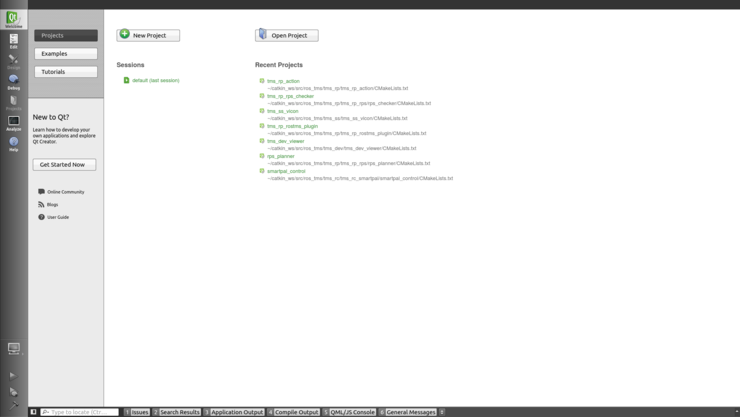
\includegraphics[width=0.8\columnwidth]{pictures/chapter2/qtcreator1.png}
\caption{QtCreator IDE}
\end{figure}

%-------------------------------------------------------------------------------
\subsubsection{ROS 패키지를 프로젝트로 불러오기}
앞서 말한바와 같이 QtCreator는 CMakeLists.txt 를 사용한다. 그렇기에 ROS 패키지는 단순히 아래와 화면의 OpenProject 버튼을 클릭하여 해당 ROS 패키지의 CMakeLists.txt 를 선택하면 손쉽게 프로젝트로 불러올 수 있다.

\begin{figure}[h]
\centering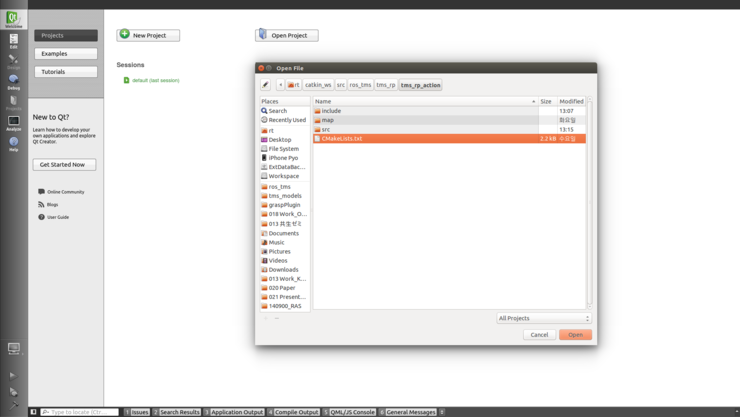
\includegraphics[width=0.8\columnwidth]{pictures/chapter2/qtcreator2.png}
\caption{QtCreator: 프로젝트 열기}
\end{figure}

%-------------------------------------------------------------------------------
\subsubsection{ROS 패키지를 프로젝트로 불러오기}
컴파일의 경우에는 단순히 Ctrl + B 로 컴파일 하면 catkin\_make 가 실행된다. 단, 빌드 관련은 해당 패키지와 같은 위치의 폴더에 새로운 폴더로 생성된다. 예를 들어 tms\_rp\_action 이라는 패키지를 컴파일하면 "build-tms\_rp\_action-Desktop-Default" 이라는 폴더에 빌드 관련이 모두 놓이게 된다. 즉,  원래는 ~/catkin\_ws/build 와 ~/catkin\_ws/devel 에 보관되어야 할 파일들이 따로 컴파일 되어 새로운 장소에 놓이게 되므로 실행을 위해서는 나중에 다시 한번 catkin\_make 를 해줘야 한다. 이는 매번 해줄 필요는 없고 개발도중에는 QtCreator 에서 개발, 디버깅을 한 후에 완료되어 실행할때만 따로 catkin\_make 를 해준다고 보면된다. 

\begin{figure}[h]
\centering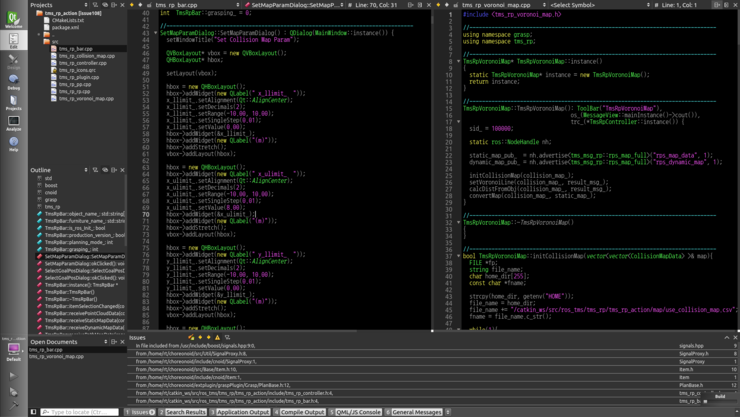
\includegraphics[width=0.8\columnwidth]{pictures/chapter2/qtcreator3.png}
\caption{QtCreator: 프로젝트 전개 모습}
\end{figure}

%-------------------------------------------------------------------------------
\section{ROS 동작 테스트}\index{ROS 동작 테스트}

%-------------------------------------------------------------------------------
\subsection{turtlesim 패키지}
일단, ROS를 설치하긴 했는데, 제대로 작동되는지 궁금하신분들을 위해 ROS에서 제공하는 간단한 예제 노드를 실행하는 방법에 대해 설명한다. 예제는 turtlesim 이라는 패캐지(노드의 묶음)로 ROS의 심볼인 거북이 모양을 한 로봇이 화면에 나타나고 키보드로 로봇의 이동을 간단히 조종해 보는 노드(프로그램)이다.

이번 강좌부터는 "노드", "패키지", "코어" 등 ROS 의 고유의 용어들이 많이 등장하는데 이번 강좌에서는 단순히 이런게 있구나 알아두기 바라며, 자세한 설명은 "ROS 강좌 : 08. ROS 컨셉", "ROS 강좌 : 09. ROS 용어" 등에서 설명하도록 하겠다. 이번 강좌는 ROS 가 문제없이 설치됨을 확인하는가 동시에, 본격적인 ROS 강좌가 들어가기 전에 몸풀기 운동 정도로 생각하자.

%-------------------------------------------------------------------------------
\subsection{roscore 실행}
새로운 터미널을 열어 다음과 같은 명렁어를 실행한다. 그러면, 모든 ROS 시스템을 관할하는 로스코어(roscore)가 실행되게 된다.

\begin{lstlisting}[language=bash]
roscore
\end{lstlisting}

\begin{figure}[h]
\centering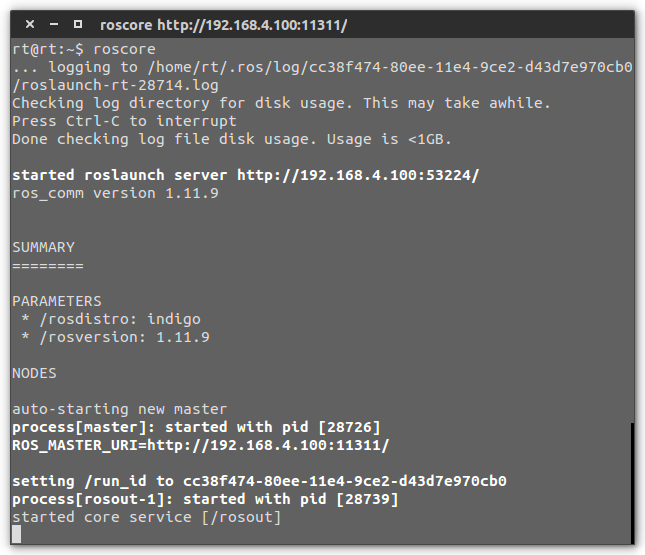
\includegraphics[width=0.7\columnwidth]{pictures/chapter2/roscore.png}
\caption{caption}
\end{figure}

%-------------------------------------------------------------------------------
\subsection{turtlesim 패키지의 turtlesim\_node 실행}
새로운 터미널을 열어 다음과 같은 명렁어를 실행한다. 그러면 다음와 같은 메시지를 보게 되며, turtlesim 패키지의 turtlesim\_node 를 실행하게 된다. 별도의 창에 파란색 바탕의 화면에 거북이 한 마리가 보일 것이다. (거북이 모양은 실행에 따라 랜덤으로 바뀌기 때문에 필자의 모양과는 다를 수 있다.)

\begin{lstlisting}[language=bash]
rosrun turtlesim turtlesim_node
[ INFO] [1378628396.169086362]: Starting turtlesim with node name /turtlesim
[ INFO] [1378628396.178989006]: Spawning turtle [turtle1] at x=[5.544445], y=[5.544445], theta=[0.000000]
\end{lstlisting}

\begin{figure}[h]
\centering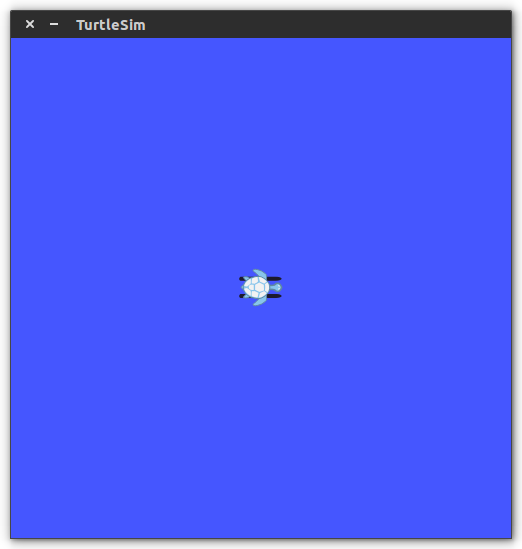
\includegraphics[width=0.5\columnwidth]{pictures/chapter2/turtlesim_node.png}
\caption{turtlesim\_node 노드를 실행한 모습}
\end{figure}

%-------------------------------------------------------------------------------
\subsection{turtlesim 패키지의 turtle\_teleop\_key 실행}
새로운 터미널을 열어 다음과 같은 명렁어를 실행한다. 그러면 다음과 같은 메시지를 보게 되며, turtlesim 패키지의 turtle\_teleop\_key를 실행하게 된다. 이 터미널 창 위에서 키보드의 화살표(← → ↑ ↓)를 이용하여 거북이를 제어하게 된다. 간단하므로 직접 해보길 바란다. 제어하게 되면 화면 속의 거북이가 움직이게 되는데, 이는 간단히 시뮬레이션이지만 실제 로봇도 이와 같은 방법으로 원격조정이 가능하게 된다.

\begin{lstlisting}[language=bash]
rosrun turtlesim turtle_teleop_key
Reading from keyboard
---------------------------
Use arrow keys to move the turtle.
\end{lstlisting}

\begin{figure}[h]
\centering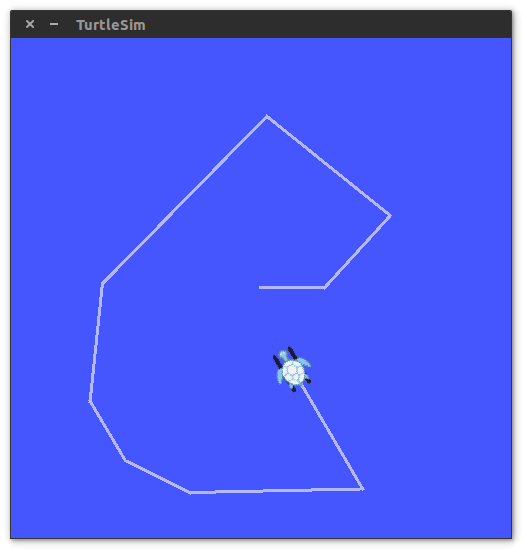
\includegraphics[width=0.5\columnwidth]{pictures/chapter2/turtlesim_node_move.png}
\caption{turtle\_teleop\_key 노드를 실행하여 화면위의 거북이를 이동시킨 모습}
\end{figure}

%-------------------------------------------------------------------------------
\subsection{rqt\_graph 패키지의 rqt\_graph 실행}
새로운 터미널을 열어 다음와 같은 명렁어를 실행한다. 그러면 rqt\_graph 패키지의 rqt\_graph를 실행하게 된다. 그 결과 다음과 같은 그래프를 볼 수 있을 것이다. 이는 현재 실행중인 노드(프로그램)들의 정보를 그래프로 볼 수 있는 노드이다.

\begin{lstlisting}[language=bash]
rosrun rqt_graph rqt_graph
\end{lstlisting}

아래의 rqt\_graph 노드는 현재 실행 중인 노드들의 정보를 볼 수 있는 GUI 형태의 노드이다. 동그라미는 노드를 의미하고, 네모는 토픽을 의미한다. 다음의 그림을 자세히 보자. /teleop\_turtle 노드로부터 화살표가 그어져 /turtlesim 으로 이어져 있다. 이는 두 노드가 실행 중 이고, 이 두 노드 간에는 메시지 통신이 이루어 지고 있다는 설명이다. 

그리고 화살표 사이의 네모박스 turtle1 토픽의 하위 토픽인 /turtle1/cmd\_vel 는 두 노드간의 토픽의 이름으로, teleop\_turtle 노드에서 키보드로 입력한 속도 명령이 turtlesim 으로 토픽을 통해 메세지(msg 데이타)가 송수되고 있다는 내용이다. 

즉, 위에서 실행한 두 노드를 이용하여 키보드 명령을 로봇 시뮬레이션에게 전달해 줬다는 내용이다. 자세한 내용은 추후에 ROS 강좌 에서 하도록 하고, 여기까지 진행이 원만히 되었다면, ROS 구동 테스트는 끝나게 된다.

\begin{figure}[h]
\centering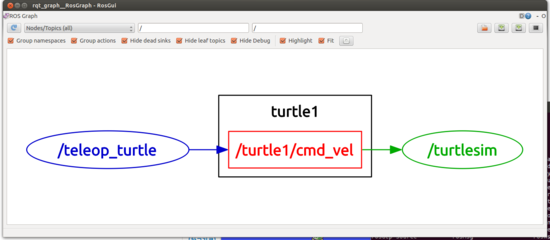
\includegraphics[width=0.8\columnwidth]{pictures/chapter2/turtlesim_node_graph.png}
\caption{노드들의 정보를 볼 수 있는 GUI 형태의 rqt\_graph 노드}
\end{figure}

%-------------------------------------------------------------------------------
\subsection{노드의 종료}

각각 실행된 roscore 및 노드는 터미널 창에서 Ctrl + c 를 눌러 종료한다.

%-------------------------------------------------------------------------------